% ============================================================
% Slides — Trabalho Final de Tópicos em IA (Grupo 2, UFPI)
% Compilar DENTRO de slides/:  pdflatex main.tex (2x)
% Tema: Metropolis + paleta e tipografia dos slides do TCC
% ============================================================
\documentclass[aspectratio=169,11pt]{beamer}

\usetheme[progressbar=frametitle, numbering=fraction]{metropolis}

\usepackage[brazil]{babel}
\usepackage[utf8]{inputenc}
\usepackage[T1]{fontenc}
\usepackage[sfdefault,scaled=0.95]{sourcesanspro}
\usepackage{booktabs}
\usepackage{amssymb,amsmath}
\usepackage{graphicx}

\graphicspath{{../results/}{.}}

% ---------- Paleta ----------
\definecolor{dsOrange}{RGB}{191,128,38}   % destaque
\definecolor{dsBlue}{RGB}{57,57,134}      % secundária
\definecolor{dsDark}{RGB}{35,38,41}
\definecolor{dsGreen}{RGB}{58,122,82}     % ganho / depois

\setbeamercolor{progress bar}{fg=dsOrange}
\setbeamercolor{alerted text}{fg=dsOrange}
\setbeamercolor{frametitle}{bg=dsDark}

% Atalho: números grandes nos slides de resultado
\newcommand{\bignum}[1]{{\fontsize{34}{38}\selectfont\fontseries{sb}\selectfont #1}}

\title{Adaptação de LLMs na prática}
\subtitle{Seis técnicas sobre o mesmo modelo e o mesmo domínio:\\
          Qwen3 nos Diários Oficiais do Piauí}
\author{Francisco Cosme Monteiro Xavier \and Heitor Andrade Moura \and
        Isaac Augusto Santana Brito \and João Pedro Monteiro da Silva Barros\\[2mm]
        {\small Grupo 2 \quad Prof.\ Raimundo Santos Moura}}
\institute{Departamento de Computação, Universidade Federal do Piauí\\
           DC/CCN072, Tópicos em Inteligência Artificial}
\date{Julho de 2026}
\titlegraphic{\hfill
\includegraphics[height=1.4cm]{logo-ufpi.png}}

\begin{document}

\maketitle

% ============================================================
% BLOCO 1 — GANCHO (2 min)
% ============================================================

\begin{frame}{O modelo parece saber}
  Perguntamos ao Qwen3-4B, sem nenhuma adaptação, 30 perguntas sobre
  atos reais dos Diários Oficiais dos Municípios do Piauí:
  \vspace{4mm}
  \begin{columns}[c]
    \column{0.48\textwidth}\centering
      similaridade semântica\\[3mm]
      \bignum{0,831}\\[2mm]
      {\footnotesize a resposta ``soa'' certa}
    \column{0.48\textwidth}\centering
      \alert{acerto factual}\\[3mm]
      \textcolor{dsOrange}{\bignum{0/30}}\\[2mm]
      {\footnotesize nenhum fato local correto}
  \end{columns}
  \vspace{5mm}
  \centering O modelo fala como um Diário Oficial,
  mas \alert{não sabe nenhum fato local}.
\end{frame}

\begin{frame}{Duas perguntas guiam o trabalho}
  \begin{enumerate}
    \item Como \alert{dar conhecimento} de um domínio a um LLM?\\
          {\footnotesize pré-treino contínuo, SFT, destilação, RAG, guardrails}
    \vspace{3mm}
    \item Como \alert{medir de verdade} o que mudou?\\
          {\footnotesize métricas que saturam, métricas que enganam,
           intervalos de confiança}
  \end{enumerate}
  \vspace{5mm}
  \textbf{Tese central}: cada técnica resolve uma coisa diferente.
  Otimizar ``o modelo'' como objetivo único esconde essa divisão
  de trabalho.
\end{frame}

% ============================================================
% BLOCO 2 — SETUP (2 min)
% ============================================================

\begin{frame}{Configuração comum}
  \begin{itemize}
    \item \textbf{Modelo}: Qwen3-4B na rodada oficial
          (aluno da destilação: 0.6B; sonda de esquecimento: 1.7B)
    \item \textbf{Dados}: DOM-PI (corpus dos Diários Oficiais) e
          docentesDC (13.762 docs rotulados por professor)
    \item \textbf{Infra}: Google Colab com GPU T4 \alert{grátis};
          QLoRA 4-bit para caber um 4B em 16 GB
    \item \textbf{Benchmarks próprios}: 30 abertas $+$ 20 MCQ (DOM-PI)
          e 100 MCQ (destilação), com distratores reais do corpus
  \end{itemize}
  \vspace{3mm}
  {\footnotesize Adapters publicados no Hugging Face; notebooks executados
   com outputs preservados como prova de execução.}
\end{frame}

\begin{frame}{Seis questões, sete notebooks}
  \begin{center}
    \small
    \renewcommand{\arraystretch}{1.15}
    \begin{tabular}{@{}lll@{}}
      \toprule
      & \textbf{Técnica} & \textbf{O que ela entrega} \\
      \midrule
      Q1 & Pré-treino contínuo (LoRA) & fluência no domínio \\
      Q2/Q3 & SFT com QLoRA & uma tarefa específica \\
      Q4 & Destilação 4B $/$ 0.6B & compressão de competência \\
      Q5 & RAG (e5 $+$ FAISS) & fatos verificáveis \\
      Q6 & Guardrails & segurança sem treino \\
      \bottomrule
    \end{tabular}
  \end{center}
  \vspace{3mm}
  O notebook 01 mede o ``antes'' comum; o 07 cruza todos os modelos
  nos mesmos benchmarks, com IC 95\%.
\end{frame}

% ============================================================
% BLOCO 3 — Q1 (2 min)
% ============================================================

\begin{frame}{Q1: pré-treino contínuo adapta sem esquecer}
  Treino de próximo token com LoRA sobre 800 documentos do DOM-PI:
  \vspace{2mm}
  \begin{center}
    \begin{tabular}{lccc}
      \toprule
      & Antes & Depois & \\
      \midrule
      Perplexidade no domínio & 7,05 & \textbf{3,77} &
        {\footnotesize queda de 47\%}\\
      Acurácia de token & 0,612 & \textbf{0,695} & \\
      \bottomrule
    \end{tabular}
  \end{center}
  \vspace{3mm}
  \textbf{Sonda de esquecimento} (1.7B): a perplexidade
  \alert{fora do domínio não sobe} (de 7,94 para 6,64).
  Adaptação \textbf{sem esquecimento catastrófico}.
\end{frame}

% ============================================================
% BLOCO 4 — Q2/Q3, A REVIRAVOLTA (4 min)
% ============================================================

\begin{frame}{Q2/Q3: SFT com QLoRA, e um resultado que assustou}
  Tarefa: \alert{atribuição de autoria} no docentesDC
  (documento $\Rightarrow$ um de 19 professores).
  Treinamos só \alert{1,48\%} dos parâmetros (33M de 2,24B).
  \vspace{4mm}
  \begin{center}
    primeira avaliação (cloze por loss média):\\[3mm]
    \bignum{0,04}\quad{\large antes}\qquad
    \bignum{0,04}\quad{\large depois}
  \end{center}
  \vspace{4mm}
  \centering A loss de treino caiu de 2,64 para 1,97\ldots\
  então \alert{quem estava errado: o treino ou a métrica?}
\end{frame}

\begin{frame}{A métrica estava errada}
  Deixando o modelo \alert{gerar} o nome (e comparando normalizado):
  \vspace{3mm}
  \begin{columns}[c]
    \column{0.48\textwidth}\centering
      antes do SFT\\[3mm]
      \bignum{0,00}
    \column{0.48\textwidth}\centering
      \alert{depois do SFT}\\[3mm]
      \textcolor{dsGreen}{\bignum{0,56}}\\[2mm]
      {\footnotesize acaso $= 0{,}05$; baseline de classe $= 0{,}24$}
  \end{columns}
  \vspace{5mm}
  O cloze por loss média tem \alert{viés de comprimento} e ranqueia mal
  nomes compostos: subestimava um modelo que acerta a maioria.
  \vspace{2mm}

  \centering\fontseries{sb}\selectfont
  A escolha da métrica pode inverter a conclusão.
\end{frame}

\begin{frame}{Q2/Q3: a prova mais forte}
  Perplexidade que o modelo atribui à \alert{resposta correta}:
  \vspace{2mm}
  \begin{columns}[c]
    \column{0.5\textwidth}
      \centering
      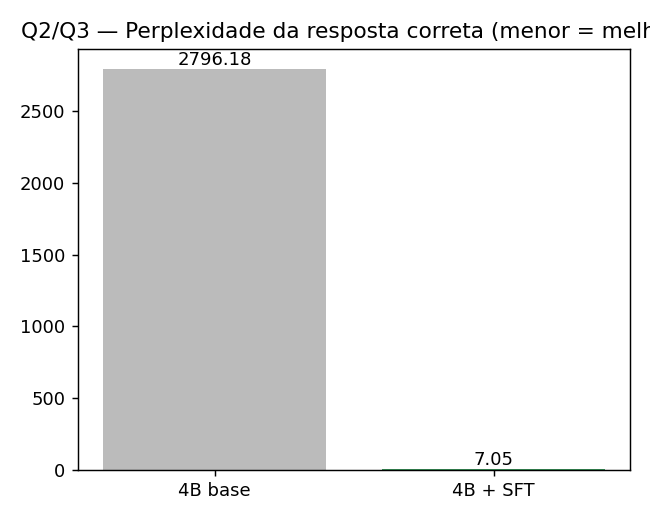
\includegraphics[width=\textwidth]{fig_sft_ppl.png}
    \column{0.46\textwidth}
      \centering
      de \bignum{2796}\\[2mm]
      para \textcolor{dsGreen}{\bignum{7,05}}\\[3mm]
      {\footnotesize queda de cerca de 400 vezes:\\
       o SFT ``gravou'' a tarefa no modelo}
  \end{columns}
\end{frame}

% ============================================================
% BLOCO 5 — Q4 (2 min)
% ============================================================

\begin{frame}{Q4: destilação é compressão}
  O professor (4B) responde prompts conceituais; o aluno (0.6B)
  faz SFT nessas respostas. Avaliação em metade \alert{disjunta}
  do benchmark (sem vazamento).
  \vspace{2mm}
  \begin{center}
    \begin{tabular}{lccc}
      \toprule
      MCQ & Professor 4B & Aluno antes & Aluno depois\\
      \midrule
      Conceitual & 0,732 & 0,659 & 0,659\\
      Factual (controle) & 0,250 & 0,200 & 0,300\\
      \bottomrule
    \end{tabular}
  \end{center}
  \vspace{3mm}
  O aluno retém \alert{cerca de 90\% da competência conceitual}
  com \alert{1/7 do tamanho}. O factual fica no acaso para todos:
  destilação transfere \textbf{como responder}, não \textbf{fato local}.
\end{frame}

% ============================================================
% BLOCO 6 — Q5 (3 min)
% ============================================================

\begin{frame}{Q5: RAG entrega o que falta, o fato}
  \begin{columns}[c]
    \column{0.52\textwidth}
      \centering
      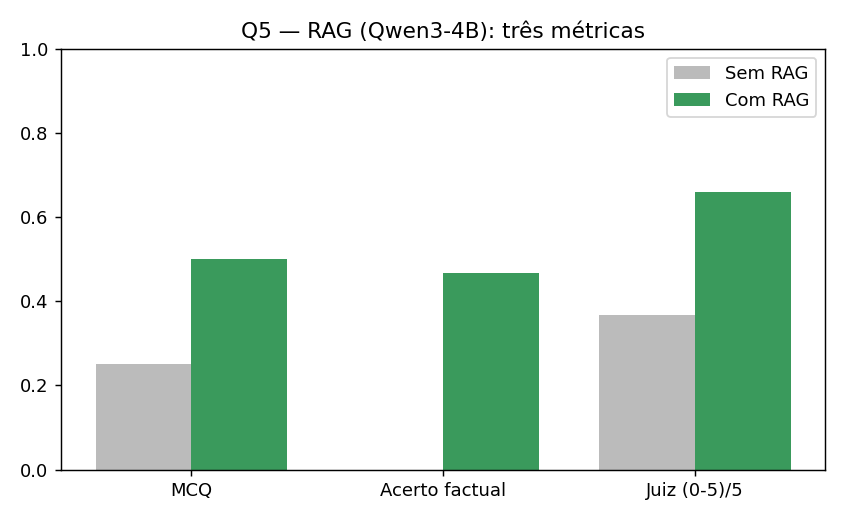
\includegraphics[width=\textwidth]{fig_rag_juiz.png}
    \column{0.44\textwidth}
      Três métricas independentes concordam:
      \begin{itemize}
        \item MCQ: 0,25 para \textbf{0,875}
              {\footnotesize (notebook 02)}
        \item acerto factual: \alert{0 para 0,433}
        \item LLM-juiz (0 a 5): 1,83 para \textbf{3,30}
      \end{itemize}
      \vspace{2mm}
      {\footnotesize O zero sem RAG é também a prova de ausência de
       contaminação: o fato local não estava decorado.}
  \end{columns}
\end{frame}

\begin{frame}{Q5: onde o RAG ainda falha}
  \begin{columns}[c]
    \column{0.52\textwidth}
      \centering
      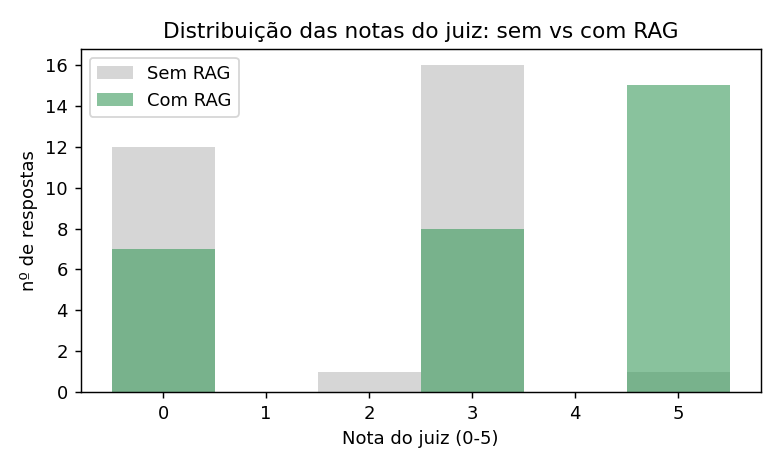
\includegraphics[width=\textwidth]{fig_juiz_hist.png}
    \column{0.44\textwidth}
      Com RAG a distribuição vira \alert{bimodal}: 0 ou 5.
      \vspace{2mm}
      \begin{itemize}
        \item recuperou o documento certo: resposta nota 5
        \item o \textit{retriever} falhou: resposta zera
      \end{itemize}
      \vspace{2mm}
      O gargalo passa a ser o \alert{recall da recuperação},
      não o modelo gerador.
  \end{columns}
\end{frame}

% ============================================================
% BLOCO 7 — Q6 + COMPARATIVA (2 min)
% ============================================================

\begin{frame}{Q6: segurança sem treinar nada}
  Moderação multi-camada: entrada, filtros, LLM e máscara de PII
  na saída, nessa ordem.
  \vspace{2mm}
  \begin{center}
    \begin{tabular}{lcc}
      \toprule
      Filtro & Acertos & Taxa\\
      \midrule
      Bloqueio de conteúdo perigoso & 18/20 & 0,90\\
      Detecção de injeção/jailbreak & 7/7 & 1,00\\
      Escopo (dentro e fora do domínio) & 8/8 & 1,00\\
      Máscara de PII (CPF, e-mail, telefone) & 6/6 & 1,00\\
      \midrule
      \textbf{Proteção geral} & \textbf{39/41} & \textbf{0,951}\\
      \bottomrule
    \end{tabular}
  \end{center}
  \vspace{2mm}
  {\footnotesize Os 2 escapes são paráfrases sem as palavras-chave:
   limite conhecido de filtros por regra (em produção, um classificador
   como Llama Guard).}
\end{frame}

\begin{frame}{Todos os modelos, o mesmo benchmark, IC 95\%}
  \begin{columns}[c]
    \column{0.58\textwidth}
      \centering
      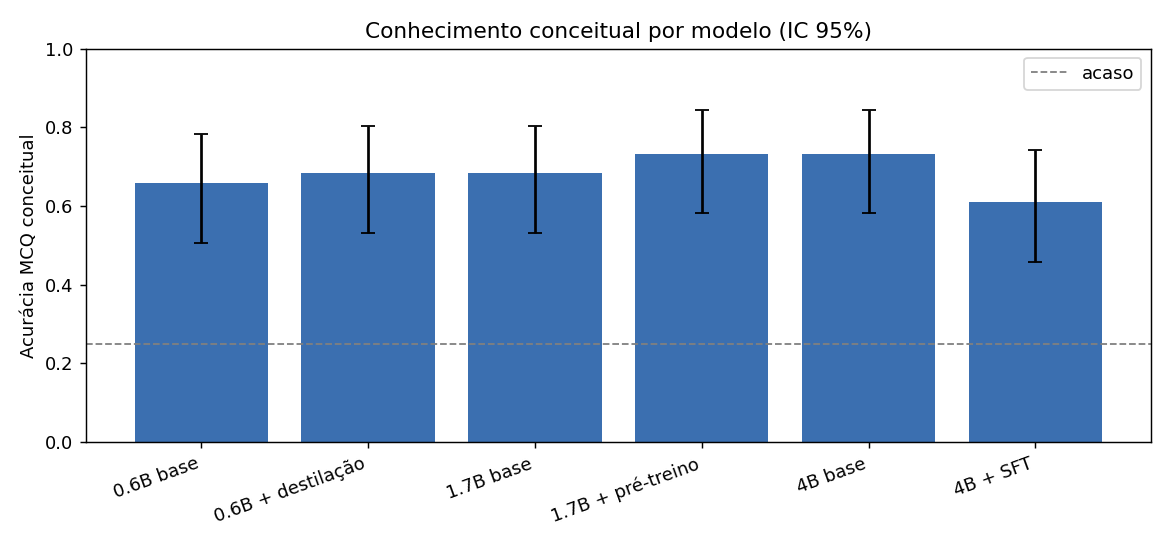
\includegraphics[width=\textwidth]{fig_mcq_ic.png}
    \column{0.38\textwidth}
      \begin{itemize}
        \item todos \alert{bem acima do acaso} (0,25)
        \item os intervalos \alert{se sobrepõem}: diferenças pequenas
              são tendência, não fato estatístico
        \item 4B$+$SFT abaixo do 4B base sugere o custo da
              especialização
      \end{itemize}
  \end{columns}
\end{frame}

% ============================================================
% BLOCO 8 — FECHAMENTO (2 min)
% ============================================================

\begin{frame}{Síntese: cada técnica resolve uma coisa}
  \begin{center}
    \renewcommand{\arraystretch}{1.2}
    \begin{tabular}{@{}lll@{}}
      \toprule
      & \textbf{Resultado} & \textbf{Leitura}\\
      \midrule
      Pré-treino & perplexidade de 7,05 para 3,77 & fluência, sem esquecer\\
      SFT/QLoRA & atribuição de 0,00 para 0,56 & tarefa específica\\
      Destilação & 90\% do professor com 1/7 & compressão\\
      RAG & factual de 0 para 0,433 & \alert{fato verificável}\\
      Guardrails & proteção 0,951 & segurança externa\\
      \bottomrule
    \end{tabular}
  \end{center}
  \vspace{4mm}
  \centering\fontseries{sb}\selectfont
  Fluência e formato vêm de adaptar o modelo;\\
  fatos vêm da recuperação; segurança vem de camadas externas.
\end{frame}

\begin{frame}{Limitações}
  \begin{itemize}
    \item \textbf{Benchmarks pequenos} (dezenas de itens):
          IC 95\% largos; reportamos incerteza em vez de
          superinterpretar
    \item \textbf{LLM-juiz da mesma família} do gerador (Qwen3-4B);
          mitigado por três métricas concordantes
    \item \textbf{RAG open-book}: o índice garante o documento-fonte;
          mede o limite superior, não recall em corpus aberto
    \item \textbf{Treinos enxutos} (T4 grátis, poucos passos):
          demonstração honesta, não estado da arte
  \end{itemize}
\end{frame}

\begin{frame}[standout]
  \normalsize
  o modelo que ``soava'' certo tirava zero em fato;\\
  medir bem importa tanto quanto treinar bem

  \vspace{6mm}
  \bignum{0 $\rightarrow$ 0,433}

  \vspace{1mm}
  {\small acerto factual com RAG, a técnica certa para o problema certo}

  \vspace{9mm}
  {\Large Obrigado! Perguntas?}
\end{frame}

% ============================================================
% BACKUP
% ============================================================
\appendix

\begin{frame}{Backup: por que a similaridade não serve como métrica}
  \begin{columns}[c]
    \column{0.55\textwidth}
      \centering
      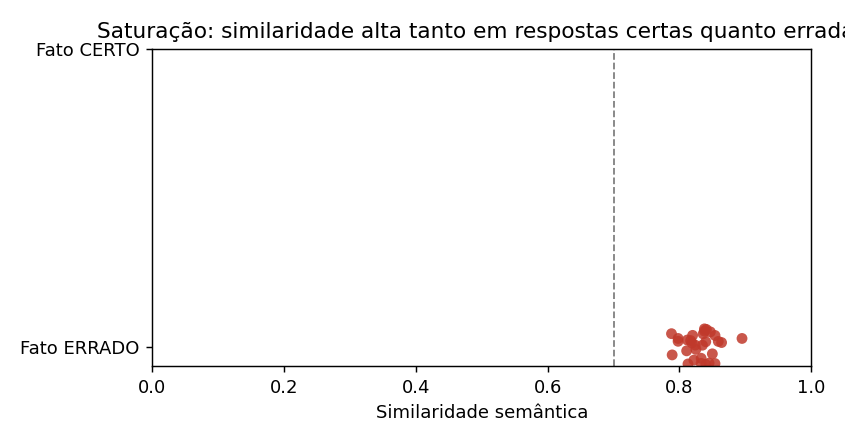
\includegraphics[width=\textwidth]{fig_saturacao.png}
    \column{0.42\textwidth}
      Respostas \alert{factualmente erradas} pontuam similaridade
      próxima de 0,85: a métrica \textbf{satura} no mesmo tema.
      \vspace{2mm}

      {\footnotesize Exemplo real: pergunta sobre a Portaria 790 de
       Teresina respondida com ``São João del Rei/MG'' teve
       similaridade 0,80.}
  \end{columns}
\end{frame}

\begin{frame}{Backup: controles de contaminação por questão}
  \begin{itemize}
    \item \textbf{Q1}: documentos-fonte do benchmark
          \alert{excluídos} do corpus de treino
    \item \textbf{Q2/Q3}: deduplicação de quase-duplicatas
          treino/avaliação; baseline de classe majoritária reportado
    \item \textbf{Q4}: treino e avaliação em metades
          \alert{disjuntas} do benchmark conceitual
    \item \textbf{Q5}: avaliação declarada \alert{open-book}
    \item \textbf{Evidência global}: o modelo cru tirou 0/30 no
          acerto factual; os fatos locais não estavam no pré-treino
  \end{itemize}
\end{frame}

\begin{frame}{Backup: o viés do cloze em 30 segundos}
  O cloze ranqueia candidatos pela \alert{loss média por token}
  do nome dado o documento:
  \begin{itemize}
    \item nomes compostos longos diluem a evidência em mais tokens
    \item tokens genéricos (``DE'', ``DA'', ``SILVA'') puxam a média
    \item resultado: candidato errado e curto vence o certo e longo
  \end{itemize}
  \vspace{3mm}
  Diagnóstico confirmado por inspeção item a item
  (\texttt{respostas\_q3.json}): em geração livre o modelo escreve
  o nome correto na maioria dos documentos do held-out.
\end{frame}

\begin{frame}{Backup: sonda de esquecimento completa (1.7B)}
  \begin{center}
    \begin{tabular}{lcc}
      \toprule
      Perplexidade & 1.7B base & 1.7B $+$ pré-treino\\
      \midrule
      Domínio (DOM-PI) & 10,46 & \textbf{8,64}\\
      Fora do domínio (docentesDC) & 7,94 & \textbf{6,64}\\
      \bottomrule
    \end{tabular}
  \end{center}
  \vspace{4mm}
  A perplexidade fora do domínio \alert{também cai}: nenhum sinal
  de esquecimento catastrófico neste regime de treino
  (LoRA, poucos passos, base congelado em 4-bit).
\end{frame}

\begin{frame}{Backup: tabela consolidada completa}
  \begin{center}
    \small
    \begin{tabular}{@{}llccc@{}}
      \toprule
      Q & Métrica & Antes & Depois & Referência\\
      \midrule
      Q1 & Perplexidade domínio & 7,05 & 3,77 & \\
      Q1 & Acurácia MCQ & 0,333 & 0,500 & acaso 0,25\\
      Q2/Q3 & Atribuição (geração) & 0,00 & 0,56 & acaso 0,05; maj.\ 0,24\\
      Q2/Q3 & PPL da resposta & 2796 & 7,05 & \\
      Q4 & MCQ conceitual (aluno) & 0,659 & 0,659 & professor 0,732\\
      Q5 & Acerto factual & 0,000 & 0,433 & \\
      Q5 & MCQ (nb 02 / nb 07) & 0,250 & 0,875 / 0,500 & benchmarks distintos\\
      Q5 & LLM-juiz (0 a 5) & 1,83 & 3,30 & \\
      Q6 & Proteção geral & -- & 0,951 & 41 casos\\
      \bottomrule
    \end{tabular}
  \end{center}
\end{frame}

\begin{frame}{Backup: reprodutibilidade}
  \begin{itemize}
    \item Repositório público:
          \texttt{github.com/heitor-am/llm-adaptation-lab}\\
          {\footnotesize notebooks executados com outputs preservados,
           resultados por item, figuras e relatório}
    \item Adapters no Hugging Face (usuário \texttt{heitor-am}):
          \texttt{qwen3-1.7b-dompi-pretrain},
          \texttt{qwen3-4b-dompi-sft},
          \texttt{qwen3-0.6b-dompi-distill}
    \item Interruptor \texttt{RETRAIN}: com \texttt{False}, os notebooks
          carregam o adapter publicado e pulam o treino
    \item Tudo roda em Colab T4 grátis; seletor \texttt{MODE} troca
          entre protótipo (1.7B) e rodada oficial (4B)
  \end{itemize}
\end{frame}

\end{document}
